\documentclass[12pt, titlepage]{article}

\usepackage{booktabs}
\usepackage{tabularx}
\usepackage{pdfpages}
\usepackage{hyperref}
\usepackage[normalem]{ulem}

\title{SFWR 3XA3: Development Plan \\ Snake 2.0}
\author{Group 34 (L03), Team Send Help
\\ Lau, Harrison (lauh3) \\ Mo, George (moz) \\ Truong, Vanessa (truonv1)
\\
\\ Professor: Dr. Asghar Bokhari}
\date{Due: September 29 2017}
\begin{document}

\maketitle
\newpage 

\tableofcontents

\newpage

\begin{table}[hp]
\caption{Revision History} \label{TblRevisionHistory}
\begin{tabularx}{\textwidth}{llX}
\toprule
\textbf{Date} & \textbf{Developer(s)} & \textbf{Change}\\
\midrule
September 26 & Harrison Lau & Set up Development plan document.\\
September 28 & Vanessa Truong & Added revison table, team meeting plan and communication plan.\\
September 29 & Vanessa Truong & Finsihed Team Meeting Plan, Communication Plan, and Member Roles, and introduction.\\
September 29 & Harrison Lau & Finished Project Schedule (Gantt Chart) and Coding Style.\\
September 29 & George Mo & Finished Technology, Git Workflow and POC.\\
November 21 & Harrison Lau & Modified for Revision 1 and completed Project Review section\\
\bottomrule
\end{tabularx}
\end{table}

\newpage


\section {Introduction}
\textbf{The Software Development Plan document will provide an outline on the project plan and schedule, and briefly elaborates on the resources and tools that the project will use.} Any confusion regarding the nature of how the project will be managed, what resources and technology the project will use, and what responsibilities a member holds will be addressed by referring to this document.

\section {Team Meeting Plan}
Team meeting times will be scheduled for \textbf{Sunday evenings on a weekly basis}. How the meeting is carried out will be a collective decision based on everyone's availability and necessity, however, they will most probably take place through the Facebook Group chat. If there are critical aspects of the project that must be discussed in person, a meeting location will be arranged at the Health Sciences Library.

During team meetings, there will be three roles: \textbf{the Chair, the Scribe, and the Moderator}. Each member will assume one of the roles for the entire semester. The roles will be discussed in further detail in the Team Member Roles sections. \textbf{Every meeting will be approximately 30-60 minutes and will follow a general structure of progress follow-up, goals for the week, work division, and open discussion.} The first 10 minutes will be dedicated for all members to discuss where they are in terms of their work and what they've accomplished. The next 10-15 minutes will be allocated to planning out objectives that we aim to accomplish by the next meeting. This part of the discussion will involve everyone's input and opinions. The objectives will then be divided amongst all members as equally as possible during the work division segment of the meeting and will be based on each member's strengths and skills so efficiency is maximized. \textbf{The final minutes of the meeting will be left for open-discussion, where questions or concerns of any team members can be addressed openly.}

In preparation for the meetings, all team members should actively participate with ideas and proposals during the discussion involving goals of the week. Otherwise, there will be no drive for the meeting. \textbf{The Chair} will be responsible for coordinating the flow of the meetings, deciding when one topic should end and another should start, and has the greatest influence on the final decisions for the project. \textbf{The Scribe} will uphold the task of recording the essential points during the meeting and logging the project accomplishments up to that time point. \textbf{The Moderator} will be responsible for all tasks not listed under the Chair or Scribe, such as refining documents before submission, and making sure all necessary files are uploaded and in the right places in the repository.
  

\section {Team Communication Plan}
Any thoughts, concerns, or inquiries regarding the project can be addressed to the team through \textbf{the Facebook Project group chat}. A team member can also personally contact another team member through Facebook or text if the topics of discussion are particular to that certain person. Although every member is considerably active on Facebook, \textbf{if reaching out to the team through the group chat proves too difficult, contact information (cell phone numbers) will be exchanged as a last resort.}

Overall, weekly team meetings will be communicated through the Facebook Project group chat. Brief meetings can take place over message but any meetings requiring the full 30-60 minute discussion will be carried out over a voice call. \textbf{Meetings held in-person will be appointed for critical milestones during the project, such as final demonstrations, programming difficulties, or program finalization.}

\section {Team Member Roles}
As mentioned above, there will be three essential roles during the project. Although the roles assignments will be permanent, members are allowed to pick up tasks that fall under other roles. 

\subsection {Chair}
The Chair (Team Leader) will be responsible for coordinating meetings and will have the biggest influence on any decisions that are made on the project. They should always have an active effort of keeping up to date with the progress of the other members, and if necessary, reassure and remind team members to fulfill the weekly objectives and assignments. Other members can voice any concerns and inquiries to the entire group, however, any ideas and proposals should be primarily addressed to the Chair, as they are the deciding factor to whether the idea gets passed or not. 

\subsection {Scribe}
The Scribe is responsible for keeping notes and logging the project progress during meetings, as well as reminding the entire team of any upcoming deadlines. They should be most aware of the itinerary for the project during the semester and update revision histories and the Gantt chart when necessary. 

\subsection {Moderator}
The Moderator will be responsible for any tasks that the Chair and Scribe do not fulfill. These responsibilities include, but are not limited to, formalizing and polishing up documents and reports prior to submission, keeping track of whether all necessary files have been pushed to the remote repository, and ensuring that the team has fulfilled all requirements for upcoming milestones.  

\section {Git Workflow Plan}
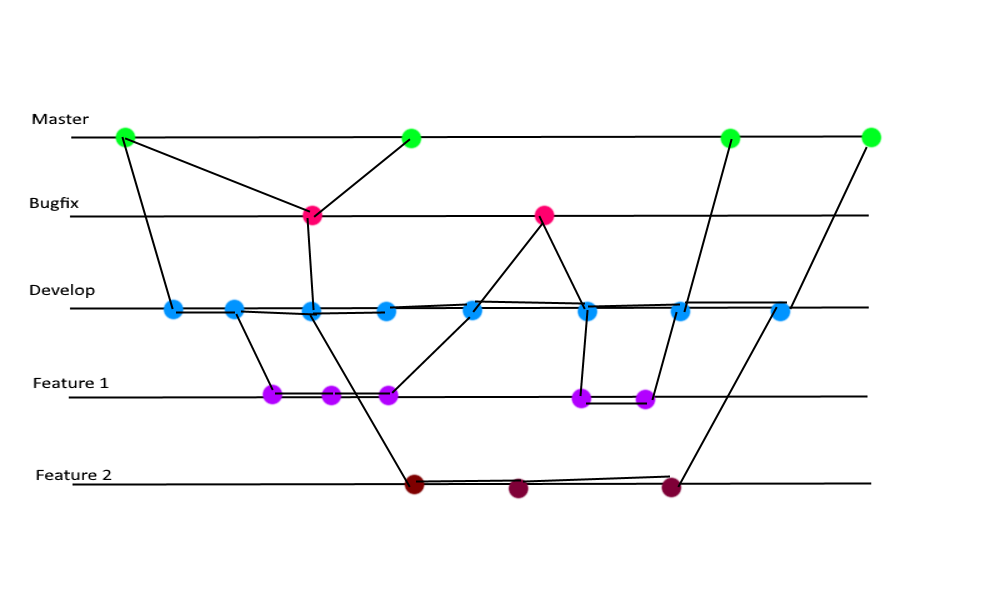
\includegraphics[scale = 0.4]{Gitworkflow.png}
\\
Above is a sample picture of a git work flow. 
\\
\\
\textbf{The repository will be centralized at the origin but subteam fetches are possible.} Our git will consist of likely at least 2 separate feature branches, likely one for map feature and the other for power-up feature.
\\
\\
\textbf{Labels} will be used throughout. As follows: 
\newline
\newline
\underline{Workflow:}
\newline
Planning, Ready, Working, Finalized
\newline
\newline
\underline{Features:}
\newline
FeaturePlan, DesignNotes
\newline
\newline
\underline{Bugs:}
\newline
MinorBug, MajorBug
\newline
\newline
\underline{Urgency:}
\newline
Urgent, Serious, Common
\newline
\newline
\textbf{Milestones} will be used throughout to reflect upon completion of key tasks.
\newline
\newline
Example milestones could include:
\newline
GameRunning, Feature1Complete, Feature2Complete, etc.
\section {Proof of Concept Demonstration Plan}

For the proof of concept, many difficulties will have to be overcome. In our eyes, \textbf{the most difficult aspect of the implementation will be the GUI} as the team has not had much experience dealing with GUIs. Basic testing of functionality should be manageable while some more intensive testing of features may prove to be more difficult. No required libraries should be difficult to install. Portability may be a risk depending on which GUI base is used. Furthermore, portability to mobile devices will be an issue. \textbf{During the demonstration we will strive to show that the required and planned aspects of the game will run and work as intended. Portability may be considered if time is sufficient.}


\section {Technology}
Based on the entire team's familiarity with the programming language, the project will be programmed in \textbf{Java} and will most likely be implemented using the \textbf{Eclipse IDE}. The testing framework to be used will be \textbf{JUnit} as it is the framework that each group member has worked with. Following the requirements for the project, all documentation will be done with \textbf{LaTeX} on any supporting text editor.  \sout{\textbf{JavaDoc}} \textbf{\textcolor{red}{Doxygen}} will be used to document code used in the project.

\section{Coding Style}
\textbf{The team will be coding in the style taught through previous courses such as SE 2S03 and SE 2AA4.} A look through Google Java Style reveals similarities between what we have been taught and what is standard. However, the Google Java Style is quite strict and does not allow for variation which is why it would be difficult to assert that our style is the same as Google's. Therefore, it would be most accurate to say our style will loosely follow Google Java Style. Considering each of the team members has taken these courses, coding style shall remain consistent throughout. Closely monitoring each other's progress will aid in preventing discrepancies.

\section{Project Schedule}
The following pages will include the pdf generated for our Gantt chart. \textbf{As the project goes on, we will be updating and adding to the chart to accurately represent and track our progress.} \textcolor{red}{The following Gantt chart is updated up to this point. Further revisions will be made in the appropriate folder.} Divisions of tasks will be distributed fairly among members and will be unanimously agreed upon.
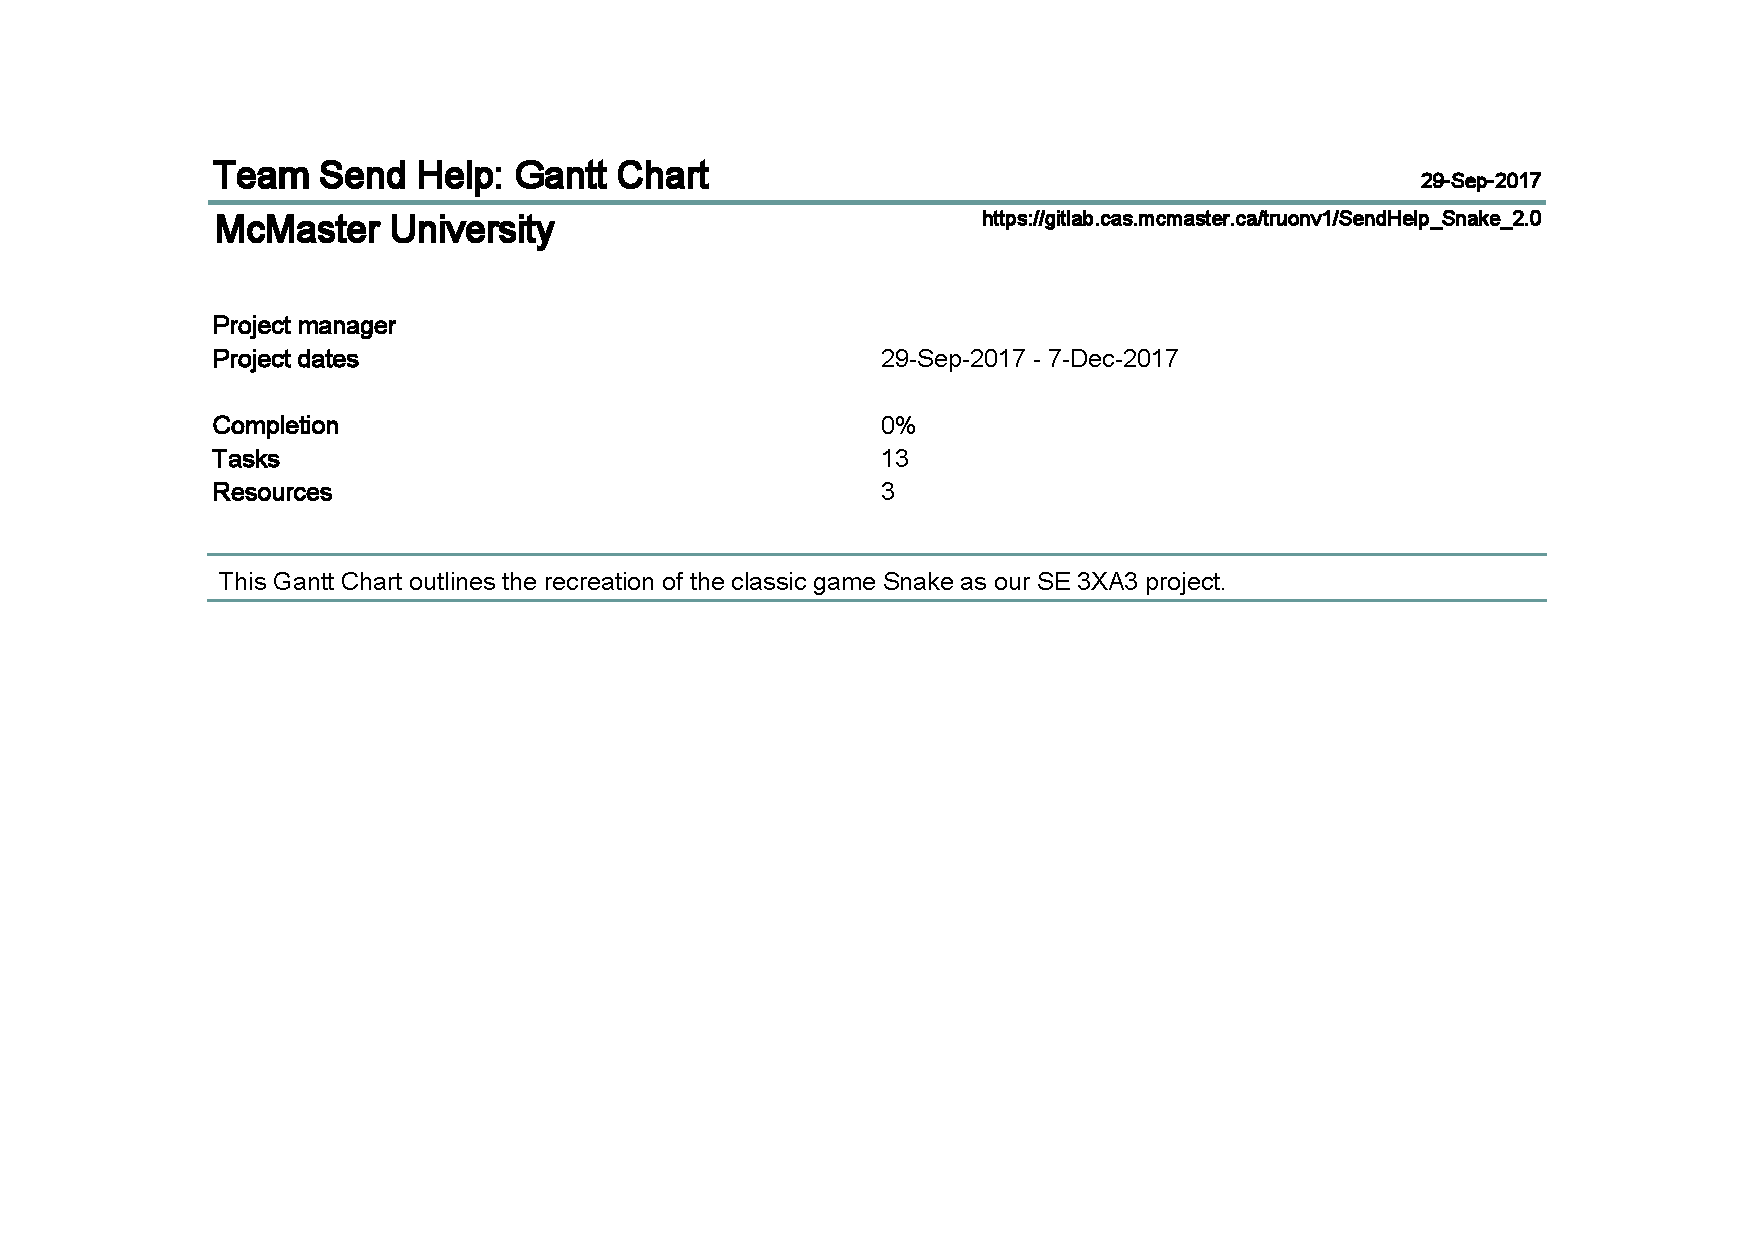
\includepdf[pages={-}]{GanttChart/SendHelp_GanttProject.pdf}

\section {Project Review}
Reflecting back on the project, most things went smoothly. All group members got along with each other. Submissions of documents and completion of relevant implementations for milestones were all done on time. However, efficient use of time to complete these documents/code was not exemplary. There were times where documents were started the day before submission and needed to be rushed.\\
In the future, proper execution of team roles is necessary (particularly the Scribe in this case) to keep the team working throughout the allotted time as opposed to doing a rushed job. That being said, procrastination isn't necessarily a group problem as it is an individual problem. 

\end{document}